\subsection{General description}

When the implemented program runs on a microcontroller, it will play an original intro sound, before giving control to the user.

He or she can then navigate between the available songs using the left and right buttons (1 and 3) on game pad, and both play, pause and resume the currently selected song using the pause button (2).
The LEDs on the game pad indicate which song is currently selected \ref{fig:systemaction}.

When the system is idling, it shuts down everything and enters deep sleep, conserving valuable energy, in turn guaranteeing a long and fruitful life for the little walkman.

The current repertoire of songs includes the original Marimba, multiple sound effects from Super Mario Bros \cite{mariobros}, and random garbage data found just outside the notes array during debugging (not available in production release).

\begin{figure}[H]
    \centering
    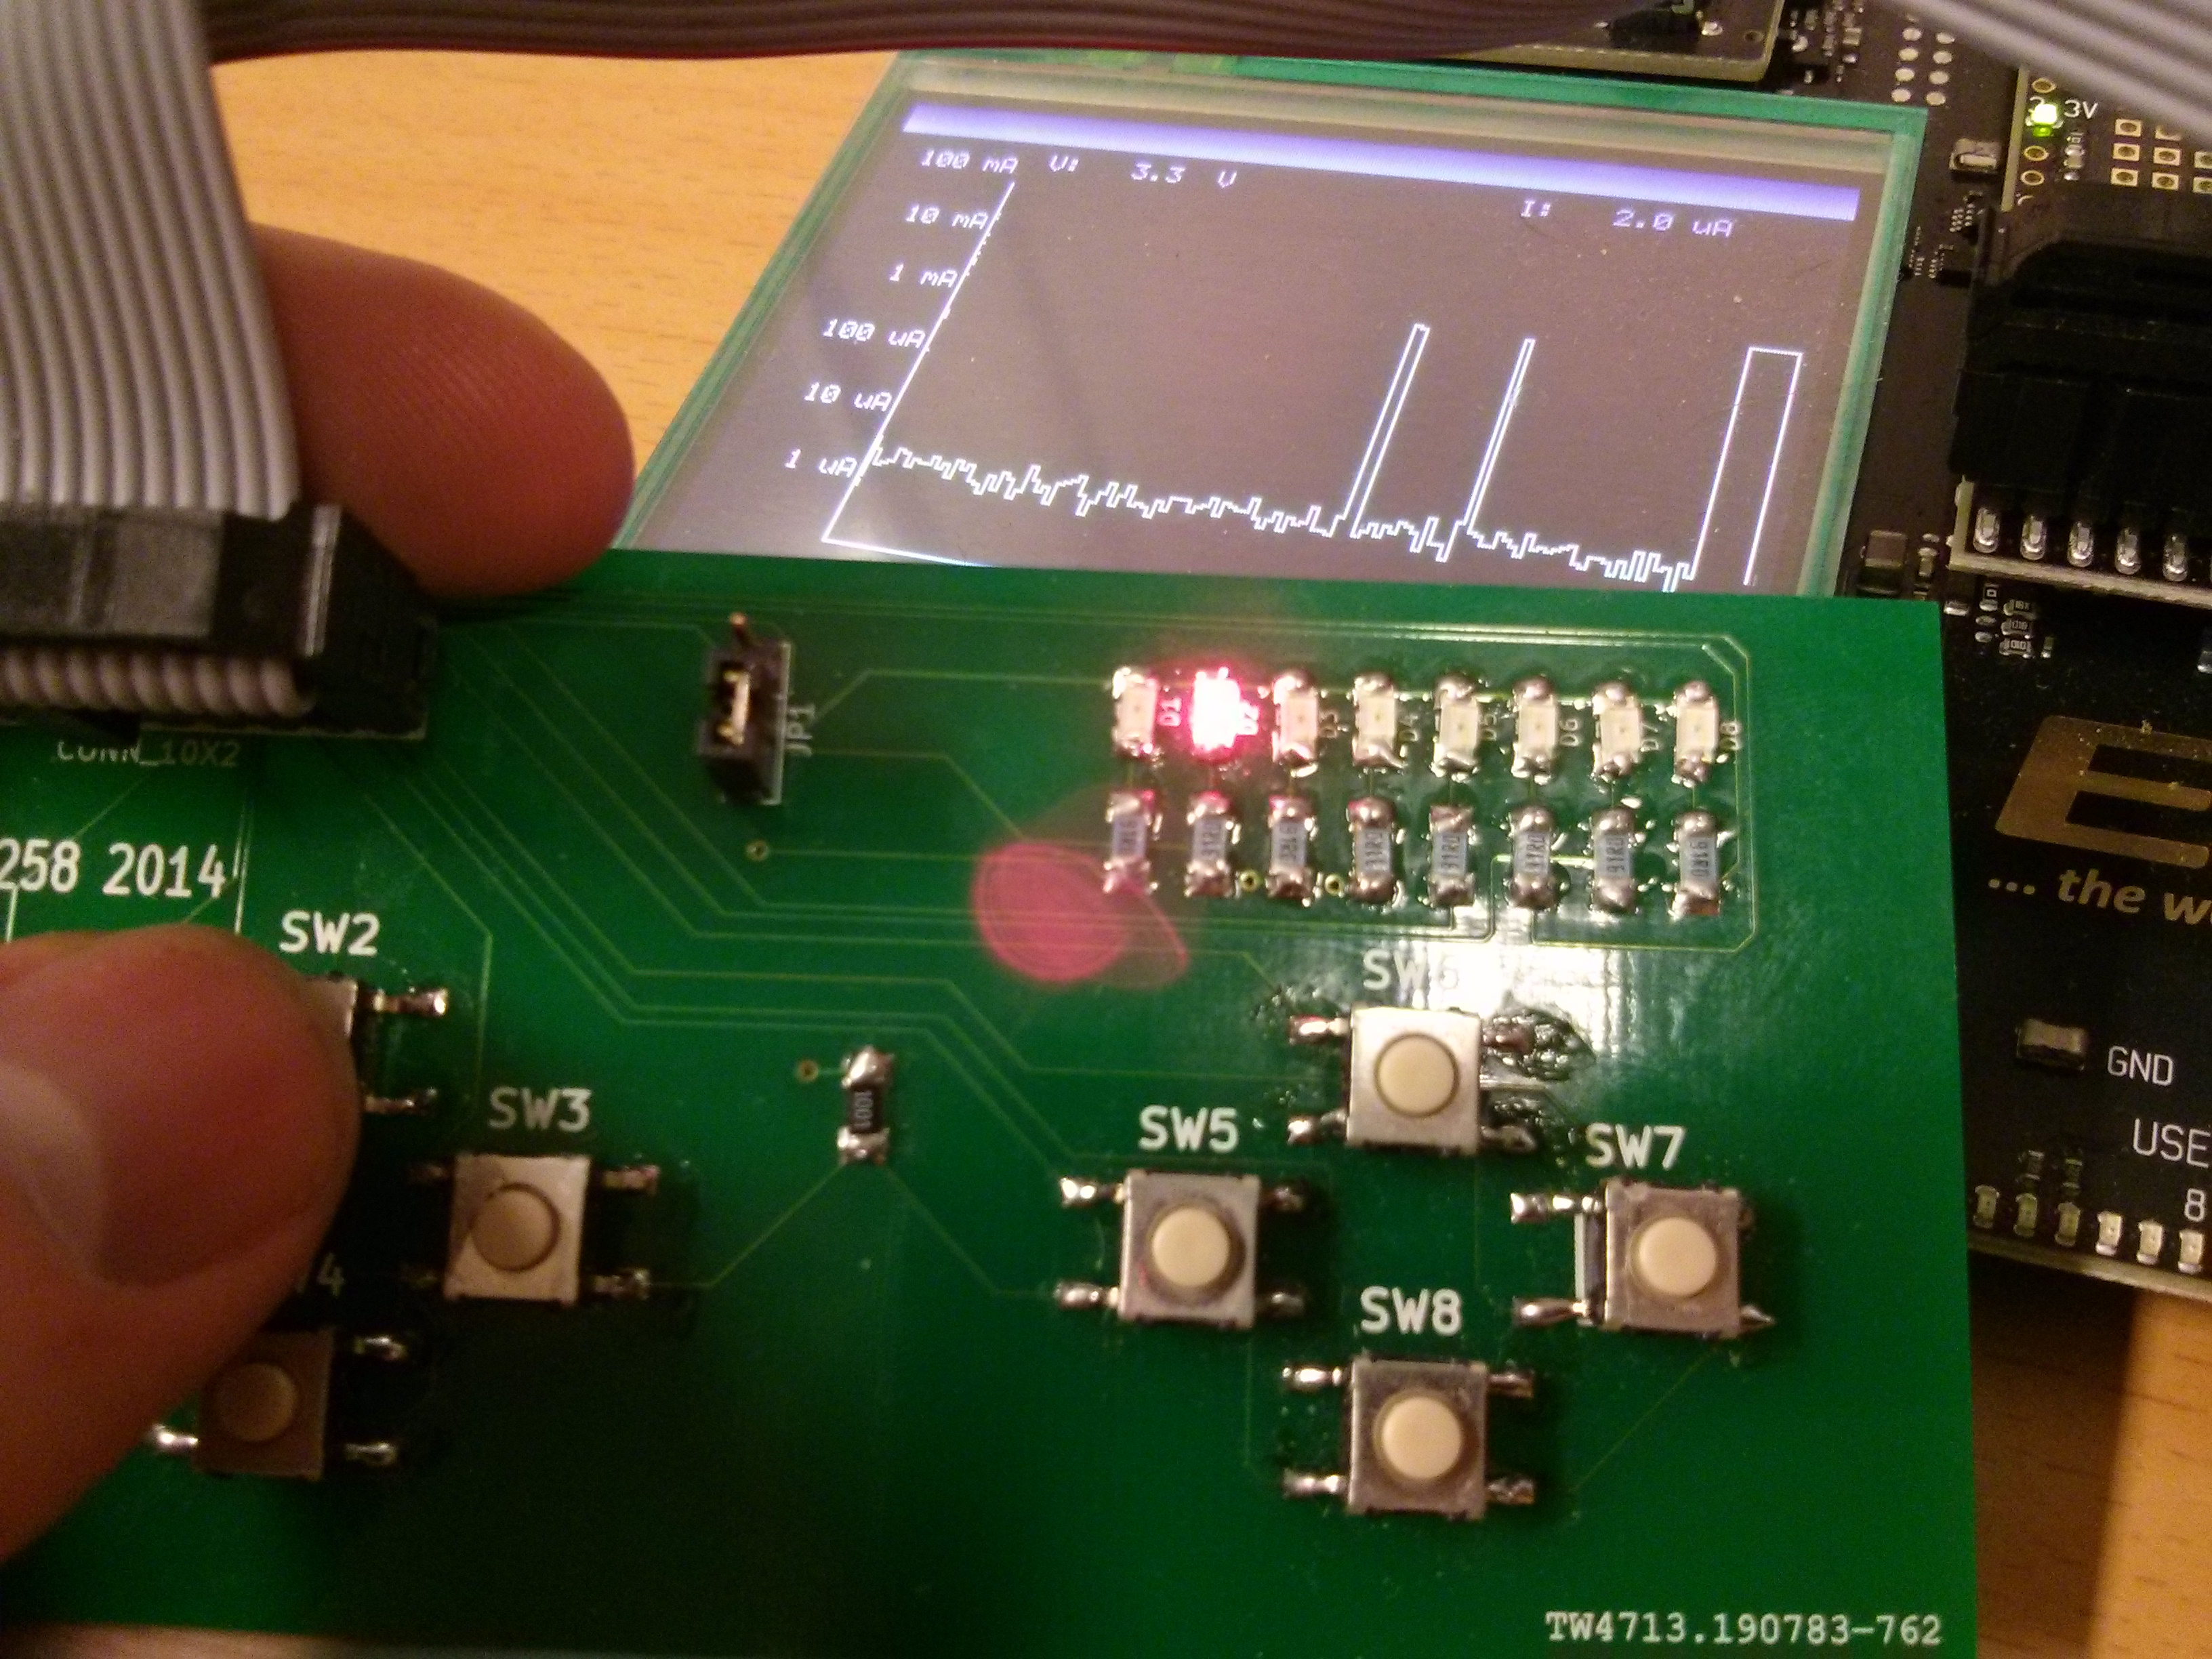
\includegraphics[width=0.75\textwidth]{figures/system-in-action.jpg}
    \caption{The system in action playing sound 2, The Fall Of Bowser from Super Mario Bros}
    \label{fig:systemaction}
\end{figure}
